% Seção: F-MET · Centralidades (RF-MET-01 a RF-MET-03; RNF-06)
% Dono: Thiago · Números: docs/plano-de-desenvolvimento/features/feature-F-MET.md, Resultados
% (comando: python benchmarks/medir_centralidade.py dados/brutos/bhtrans.zip --exato;
% execução de 16/11/2026; JSON em benchmarks/resultados/). Condensada em 20/11.
\subsection{Centralidades}\label{sec:F-MET}

A página Centralidades responde quais paradas mais importam para a rede, sobre $G_P$: grau de
entrada e de saída e intermediação de Brandes~\cite{brandes2001} por tempo, com ranking,
distribuição de graus e mapa de calor (Figura~\ref{fig:centralidades}). $G_P$ foi escolhida
porque em $G_E$ a parada vira várias plataformas e a centralidade se dividiria entre elas; o
grau conta só as arestas de viagem. Os graus custam $O(V + E)$ e o Brandes exato,
$O(V(V + E)\log V)$; a página usa a amostragem de Brandes e Pich~\cite{brandes2007} (RNF-06),
com $k$ origens sorteadas com semente fixa e erro padrão $N s_v \sqrt{(N-k)/(Nk)}$ por parada.
Os testes conferem graus e intermediação exata contra o NetworkX em grafos aleatórios e, em
grafos pequenos, que a média da estimativa sobre todas as amostras é o valor exato.

No feed de 11/11 ($V = 9{.}660$, $E = 122{.}799$), 75\% das paradas têm um único trecho de
ônibus saindo delas. O Brandes exato levou 44~min; as cinco paradas mais centrais estão na
Avenida Presidente Antônio Carlos e as cinco seguintes no Anel Rodoviário. Com 25, 50, 100 e
200 origens sorteadas (semente 2026), a estimativa levou 5,2, 15,8, 23,0 e 45,6~s, e o erro
relativo mediano nas 100 paradas mais centrais caiu de 18,6\% para 12,2\%, 8,5\% e 6,1\%, com o
exato a até dois erros padrão em 97\% a 100\% delas; com 50 origens, o padrão da página, 9 das
10 mais centrais coincidem com as do exato (Intel Core 5 120U). \textbf{Limitação.} A centralidade é da
rede estrutural, sem espera nem horário. O erro padrão só é confiável nas paradas centrais: nas
de valor pequeno o intervalo de dois erros padrão contém o exato em apenas 46\% das paradas com
$k = 50$, por isso a página mostra o erro só no ranking.

\begin{figure}[t]
\centering
\begin{minipage}[t]{0.47\linewidth}
  \centering
  \includegraphics[width=0.72\linewidth]{centralidades}
  \caption{Página Centralidades: intermediação estimada com 50 origens e mapa de calor dos 10\%
  mais centrais; os círculos são as dez primeiras.}
  \label{fig:centralidades}
\end{minipage}\hfill
\begin{minipage}[t]{0.47\linewidth}
  \centering
  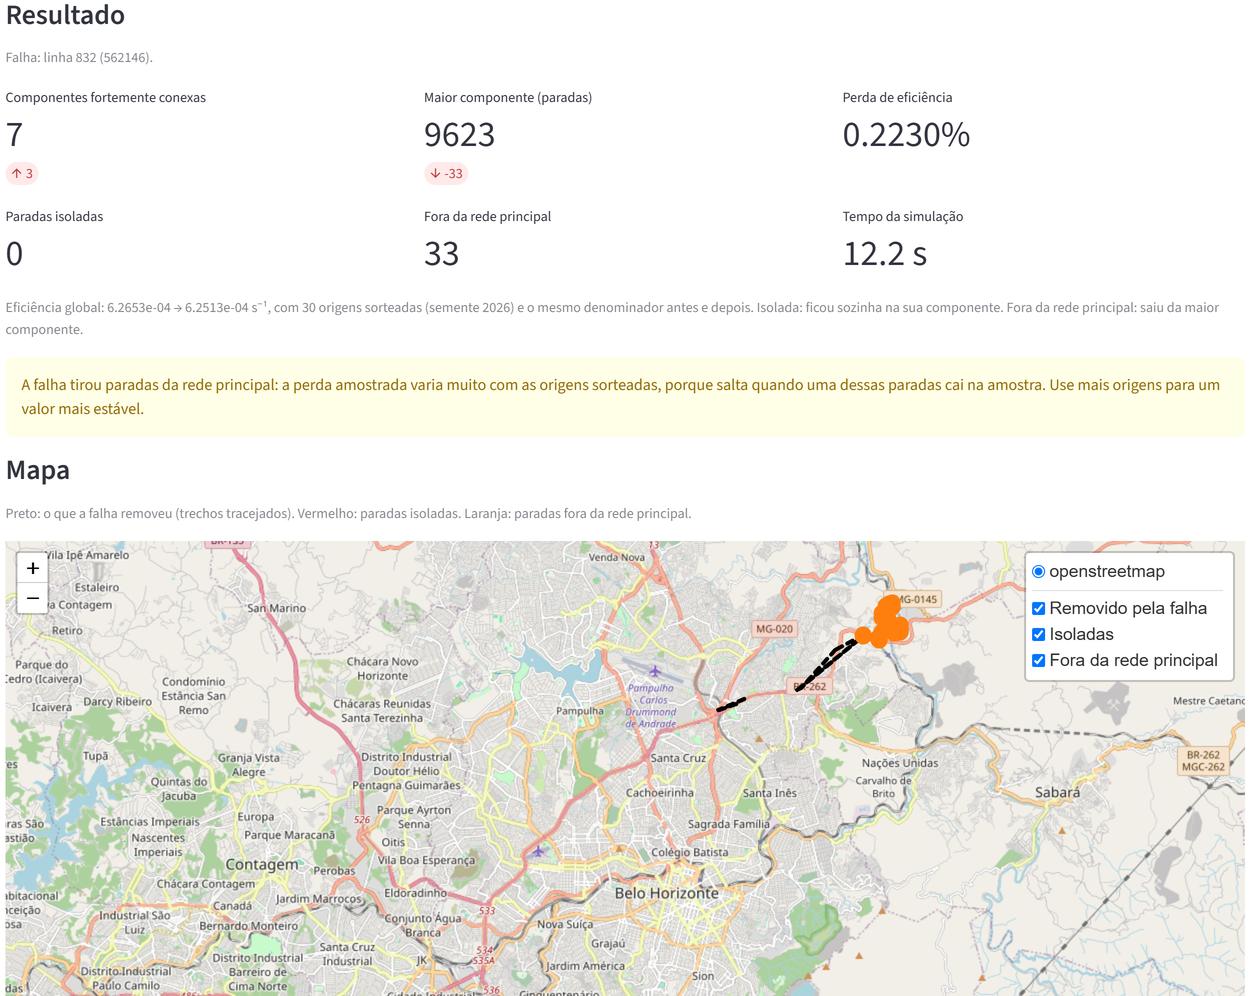
\includegraphics[width=\linewidth]{figuras/falhas-linha-832.png}
  \caption{Página Falhas: retirada da linha 832 (30 origens). As 33 paradas em laranja saem da
  rede principal; a perda exibida (0,22\%) é amostrada, e a exata é 0,50\%.}
  \label{fig:falhas}
\end{minipage}
\end{figure}
